\documentclass{article}


\usepackage{PRIMEarxiv}

\usepackage[utf8]{inputenc} % allow utf-8 input
\usepackage[T1]{fontenc}    % use 8-bit T1 fonts
\usepackage{hyperref}       % hyperlinks
\usepackage{url}            % simple URL typesetting
\usepackage{booktabs}       % professional-quality tables
\usepackage{amsfonts}       % blackboard math symbols
\usepackage{nicefrac}       % compact symbols for 1/2, etc.
\usepackage{microtype}      % microtypography
\usepackage{lipsum}
\usepackage{fancyhdr}       % header
\usepackage{graphicx}       % graphics
\graphicspath{{media/}}     % organize your images and other figures under media/ folder
\usepackage{algorithm}
\usepackage{algpseudocode}
\usepackage{amsmath}
\usepackage{amsfonts}
\usepackage{enumitem}

%Header
\pagestyle{fancy}
\thispagestyle{empty}
\rhead{ \textit{ }} 

% Update your Headers here
\fancyhead[LO]{Topology Protocol: A Distributed System Protocol for the Open Metaverse}
% \fancyhead[RE]{Firstauthor and Secondauthor} % Firstauthor et al. if more than 2 - must use \documentclass[twoside]{article}



  
%% Title
\title{Topology Protocol: A Distributed System Protocol for the Open Metaverse}

\author{
 Thomas (Hsea-Ching) Hsueh \\
 Topology \\
 gg@topology.gg \\
 @guiltygyoza
}


\begin{document}
\maketitle


\begin{abstract}

We present Topology Protocol, a distributed system protocol designed for the Open Metaverse. The Open Metaverse is a programmable medium that enables real-time multi-user, interoperable, and censorship-resistant applications on open decentralized networks. To unlock a new phase of human productivity and collaboration, this new medium requires a distributed system protocol that is credibly neutral and scalable. It must support billions of equal participants interacting in real time at negligible costs while preserving user autonomy and privacy — fundamental needs in human interactions. To meet such requirements, we introduce a new abstraction called Conflict-free Replicated Objects (CRO) and the concept of decentralized Random Access Memory (dRAM). CROs are composable programmable objects that can be subscribed to as PubSub groups on open P2P networks. They can be mutated in real time concurrently while avoiding the costs of coordination, leveraging the properties of Conflict-free Replicated Data Types (CRDTs). Hash graphs provide CROs with causal ordering and immunity to Sybil attacks. The Topology Protocol specifies methods for CRO interaction and their corresponding behavior on P2P networks. Utility, scalability and security aspects such as snapshot, compaction, verifiability, access control and equivocation tolerance are addressed. Nodes that implement the Topology Protocol form an open ephemeral P2P network, maintaining CRO states at the edge for immediate access, and in sync across all subscriber nodes. Summarizing its capabilities, we refer to this P2P network as a dRAM, a new kind of decentralized network powering distributed programs that are lock-free concurrent. CROs on dRAM will be able to interoperate with blockchains and open standards at other layers of the computing stack, advancing the landscape of world-scale distributed computing and becoming a key building block at the foundation of the Open Metaverse.
\end{abstract}


% keywords can be removed
\keywords{CRDTs \and hash graphs \and Byzantine fault tolerance \and peer-to-peer networks \and threshold logical clock}

\section{Introduction}
Multi-user applications on the Internet largely rely on centralized intermediaries to mediate user interactions. While this architecture has seen tremendous success, it suffers a number of problems. Intermediaries dictate who can access what applications when and how, limiting user agency and autonomy. Interoperability among applications is rarely possible because most intermediaries operate on the business model of building and protecting their own network effects.

The Open Metaverse must operate on open decentralized networks \cite{SIGGRAPH}. The network architecture should be horizontally scalable. It must allow billions of participants to interact in real time at negligible costs. New multi-user software can be deployed, discovered, and accessed, completely free of censorship. As such, the Open Metaverse is much broader than video games and will maximize the freedom, creativity, and productivity of humanity on the Internet.

Blockchains laid the foundation for trust-minimized ownership and censorship-resistant multiplayer software on open decentralized networks. However, their reliance on Byzantine consensus mechanisms creates limitations in speed and costs. Operating under the strict serializability model, most modern blockchain networks require global coordination among their geo-distributed nodes to reach consistency. Yet, light only travels a few inches per clock cycle of a modern CPU. Relying on global coordination over the Internet makes the transaction throughput of blockchains heavily communication-bound. To tolerate Byzantine faults, most modern blockchains employ expensive Sybil countermeasures \cite{Tendermint,Casper}, creating price floors on transaction fees to pay node operators and limiting these systems to financial use cases.

Various approaches to the blockchain scalability problem exist, yet none of them address the fundamental issue of coordination costs. One approach is to shard the network by applications \cite{Cosmos, RGB}. Another approach is to batch total-ordered blocks of transactions at rollups and submit their commitments and proofs on blockchains \cite{Rollup}. However, the transaction throughput of each shard or rollup remains heavily communication-bound.

In this paper, we sketch out a solution that leverages the concurrency, composability, and local-first \cite{LoFi} properties of Conflict-free Replicated Data Types (CRDTs) \cite{CRDT}. We propose Topology Protocol, a protocol dedicated to enabling applications that are real-time multiplayer, sovereign, and running on open P2P networks. We introduce Conflict-free Replicated Objects (CRO), a new abstraction for building multiplayer programs at ease and making them accessible on the P2P network. We explore how CROs can be applied to social graphs for social media applications, and multiplayer physics simulations with elastic collision constraints. We discuss various aspects that impact the flexibility, scalability and security of CROs, including how they can produce verifiable compacted snapshots for interacting with blockchains. Nodes that implement Topology Protocol form an ephemeral P2P network that keeps CRO states next to local compute on the edge, effectively forming a decentralized Random Access Memory (dRAM). Interoperating with open standards and protocols at other layers of the stack, Topology Protocol aims to grow into the de facto distributed system protocol of the Open Metaverse.

\section{Conflict-free Replicated Data Types}
\label{sec:headings}

Conflict-free Replicated Data Types (CRDTs) encapsulate coordination-free replication strategies and expose the application programming interface (API) of ordinary data types. Replicas of the same CRDT can progress independently. They do not require locks for synchronization. Conflicts caused by concurrent operations are automatically resolved by rules as part of the specification of the type. As a result, all replicas are guaranteed to converge eventually without ever having to coordinate.

CRDTs are expressive. One approach is to make complex CRDTs from scratch. Although notoriously tricky to get right, correct CRDTs exist for indexed sequence types \cite{Lseq, RGA, YATA, Fugue}, XML \cite{XML-CRDT}, and JSON \cite{JSON-CRDT}. Another approach is to make complex CRDTs through class composition. A class whose fields are all typed by CRDTs, and whose methods access its fields only through the public methods of their types, is itself a CRDT.

\section{Conflict-free Replicated Objects}
\label{sec:headings}

The primary abstraction of Topology Protocol is \textit{Conflict-free Replicated Object} (CRO). CROs are composable programmable objects that can be updated in real time concurrently and subscribed to as publish/subscribe (PubSub) groups on open P2P networks.

Each CRO is an instance of a \textit{blueprint}. A blueprint has two main components:
\begin{enumerate}
    \item States: Each state is typed with either a built-in CRDT recognized by the protocol, or by another blueprint through class composition.
    \item Functions: A function may read and \textit{monotonically mutate} (\textit{i.e.,} inflate) the states. All function signatures are specified in the blueprint's Application Binary Interface (ABI).
\end{enumerate}
Additionally, a \textit{merge} function must be defined for merging the states of an external replica with the local states. This merge function must be commutative, associative, and idempotent for convergence purposes. Developers can create blueprints in their programming language of choice. These blueprints can then be compiled into suitable bytecode formats for execution by nodes implementing the protocol.

\section{Causal ordering}
\label{sec:headings}

To further enhance the expressivity of CROs, we introduce causal ordering among their operations. This ordering allows for more complex relationships between operations. Causal order is a partial order that can be enforced in a distributed system without coordination. This differs from the total order in systems that offer strict serializability, which requires coordination. Given an operation history of a CRO, its state is derived from applying the operations in a linear order obtained from topological sort that preserves the causal order.

Approaches such as vector clocks and version vectors exist for capturing causality in distributed systems. However, these approaches are vulnerable to equivocation, making them unsafe in the presence of Byzantine actors. We need a way to provide causal ordering while tolerating Byzantine faults.

\subsection{Hash graphs}

We propose a solution based on hash graphs \cite{BEC, BFT-CRDT, Merkle-CRDTs, Blocklace}. The hash graph approach works by encoding an operation history in a directed acyclic graph, where the edges represent \textit{causal dependency reporting} among the operations, and vertices contain both operations and the hashes of their causal dependencies.

Notationally:
\begin{enumerate}
    \item Let $u$ be an update operation. Given two operations $u_1$ and $u_2$, if $u_2$ reported $u_1$ as its causal dependency, $u_2$ must have happened-after $u_1$. In the corresponding hash graph, there is an arrow pointing from $u_2$ to $u_1$, or $u_2 \rightarrow u_1$.
    \item Let $h(\cdot)$ be a suitable hash function.
    \item Let $\textbf{F}$ be the hash graph's \textit{frontier}, or the set of vertices whose operations are currently not the dependencies of any other operation. Let $\textbf{F}^*$ be the \textit{hashed frontier}, or $\{h(v) | v \in \textbf{F}\}$.
    \item Let $\textbf{O}$ be the hash graph's \textit{origin}, or the set of vertices whose operations do not causally depend on any other operation.
    \item For an operation, let $\textbf{D}$ be the set of hashed vertices that are its causal dependencies. For a newly generated operation $u$, its $\textbf{D}$ equals $\textbf{F}^*$ at the time of generation.
    \item Attached to the origin of a hash graph is the \textit{original state} of the CRO, or its state before applying any of the operations in the hash graph.
\end{enumerate}
We can then define a vertex of a hash graph as containing the tuple $(u, \textbf{D})$. The collision resistance of $h(\cdot)$ ensures that the hash graph contains no cycles. Figure 1 shows an example of a hash graph.

\begin{figure}[htp]
    \centering
    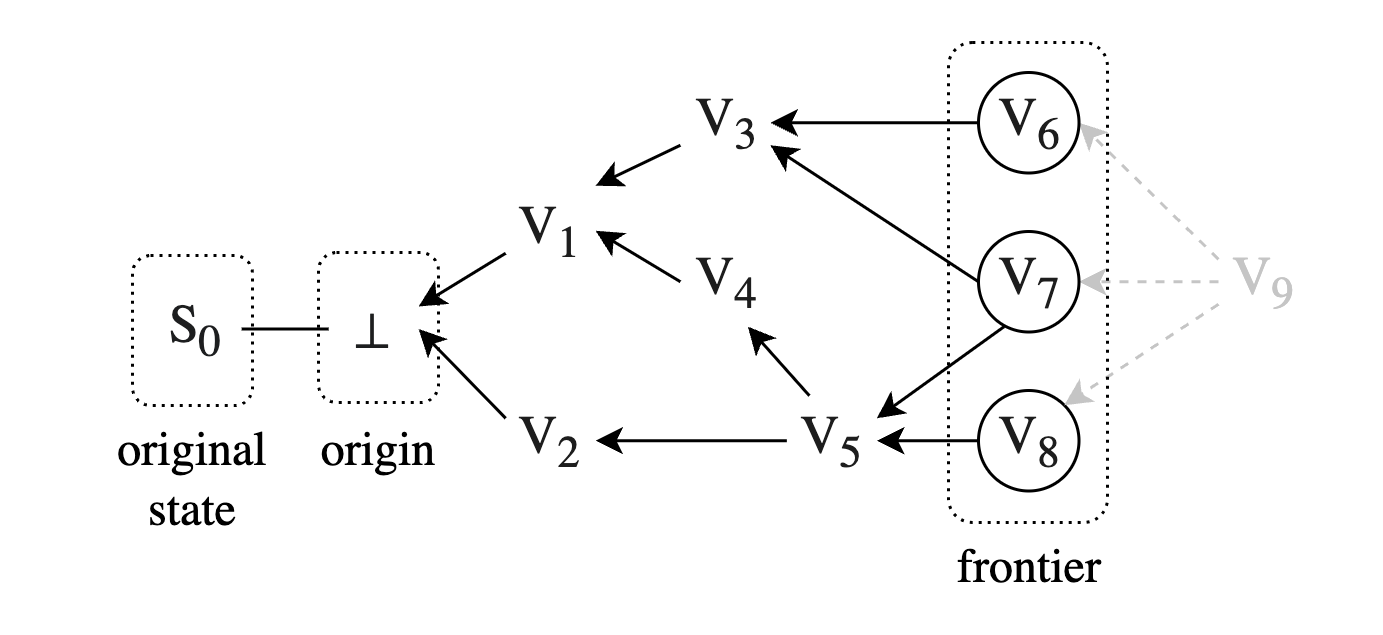
\includegraphics[width=10cm]{fig1}
    \caption{A hash graph of a CRO for illustration purposes. Given this hash graph, vertex $V_7$ should contain $(u_7, \{h(V_3),h(V_5)\})$. The vertices in the frontier $\textbf{F} = \{V_6, V_7, V_8\}$ are circled. The origin $\textbf{O}$ contains only one vertex, $\bot$, which carries a null operation. For the next vertex to be added to the graph, $V_9$, its causal dependencies should be $\textbf{F}^* = \{h(V_6), h(V_7), h(V_8)\}$. The original state of this CRO is $S_0$.}
    \label{fig:1}
\end{figure}

\begin{figure}[htp]
    \centering
    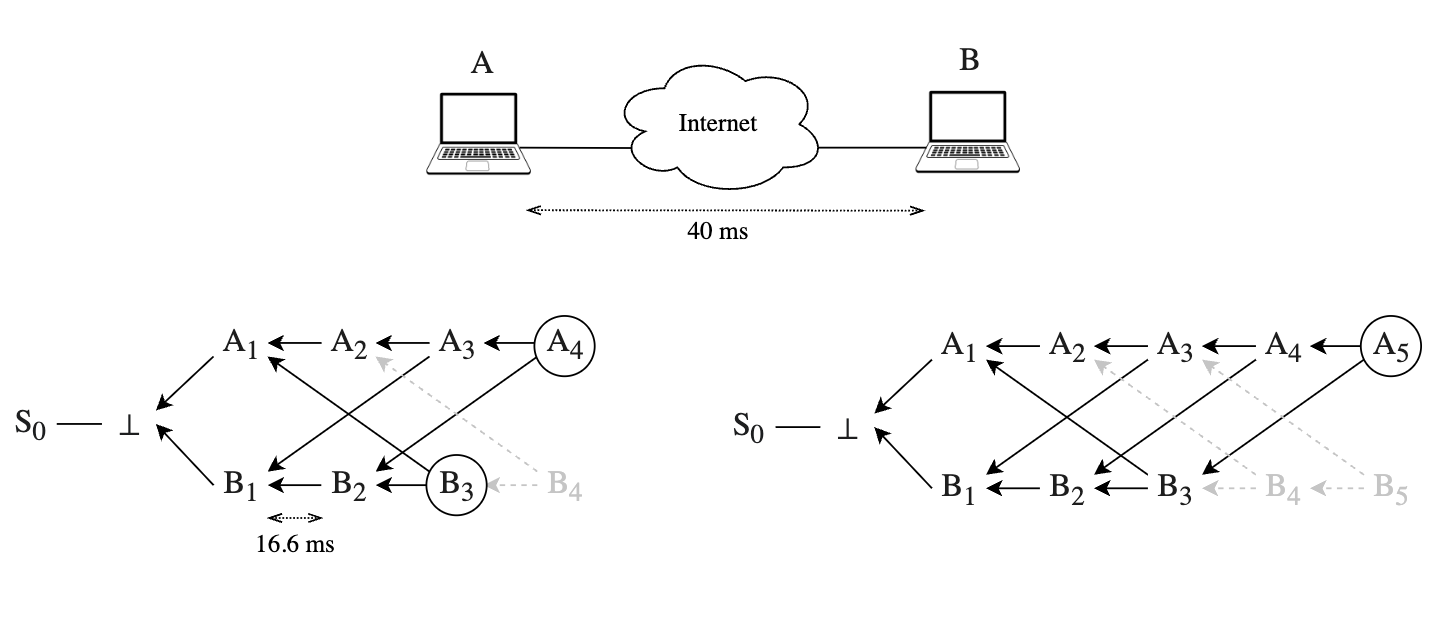
\includegraphics[width=16cm]{fig2}
    \caption{The hash graphs of node A in a hypothetical system immediately before and after A generates vertex $A_5$. Node A has not learned about the grayed out vertices, $B_4$ and $B_5$.}
    \label{fig:2}
\end{figure}

Using this approach, when two nodes synchronize their operation histories of the same CRO, they effectively merge their hash graphs. Having matching $\textbf{F}^*$ implies having equivalent hash graphs. Operations whose reported causal dependencies are unrecognized by honest nodes will not be added to their hash graphs.

As another example, consider a distributed system comprising node A and B, separated by a network delay of 40 ms. Both nodes start from the same initial state, denoted by $\bot$. Each node generates 60 operations per second ($\approx$16.6 ms between consecutive operations), a standard frame rate for games, and reconciles its hash graph with the other node as fast as the network conditions permit. Figure 2 shows the hash graphs at node A immediately before and after A generates vertex $A_5$.

This approach is immune to Sybil attacks. As long as honest nodes form a connected subgraph in the P2P network, the system is able to function correctly. This allows CROs to tolerate arbitrarily many Sybil actors, hence the immunity. In contrast, systems with global Byzantine consensus functions correctly only if less than one third of the nodes are faulty. No expensive countermeasures such as Proof of Work or Proof of Stake are involved, making the costs of transacting with CROs practically zero.

\subsection{Concurrency semantics}
Equipped with causal ordering, we now have a notion of concurrency. Two operations can be comparable (\textit{i.e.} one happened after the other) or incomparable (\textit{i.e.} they are concurrent to each other). For operations that happened concurrently but do not commute, the order at which they are serialized and executed impacts the CRO state. The \textit{concurrency semantics} of a CRO define its behavior in the presence of concurrent operations that are not commutative.

\begin{figure}[htp]
    \centering
    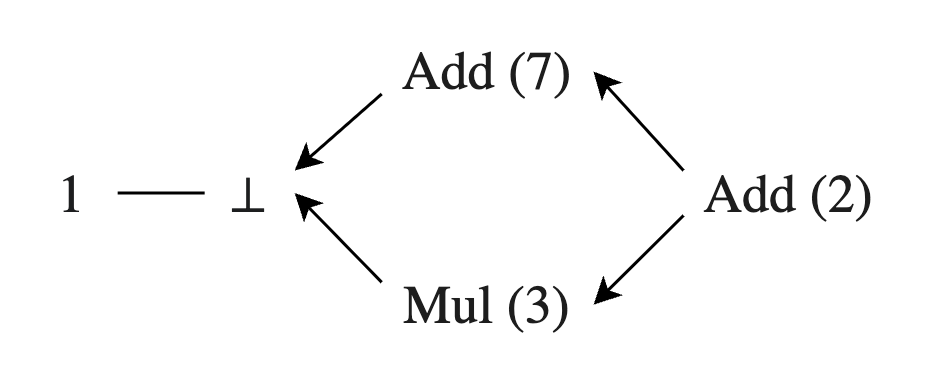
\includegraphics[width=7cm]{fig3}
    \caption{A hash graph for the register CRO that accepts addition and multiplication.}
    \label{fig:3}
\end{figure}

Consider a register CRO that holds a single integer and accepts two types of operations:
\begin{enumerate}
    \item $Add(x)$: adds $x$ to the current value
    \item $Mul(x)$: multiplies the current value by $x$
\end{enumerate}

However, integer addition and multiplication do not commute. Figure 3 shows a hash graph for this register. We can see two possible execution orders:
\begin{enumerate}
    \item $(1+7)*3+2 = 26$
    \item $(1*3)+7+2 = 12$
\end{enumerate}

To resolve this ambiguity, we can introduce the following concurrency semantics to the CRO: addition goes first in case of concurrency. With this rule, every honest replica of this hash graph would arrive at $26$ as its final state.

\section{Signaling}
\label{sec:headings}

Having established how individual CROs function, we now turn to how these objects interact with each other. CROs interact by \textit{signaling}, a CRO-level term to differentiate from messaging at the network layer. A signal originates from an operation at the sender CRO. It then materializes into an operation at the receiver CRO. For causality to work, a signal needs to specify its causal dependencies in both the sender CRO and receiver CRO's hash graphs. This means the node that intends to send a cross-object signal needs to have the hash graphs of both the sender and receiver CROs locally. This requirement creates challenges in scalability, as nodes must maintain and synchronize multiple hash graphs simultaneously. The safety and scalability of cross-object signaling remain an active area of research.

Figure 4 illustrates a cross-object signal diagrammatically, where the signal “glues” together its originating operation on the sender CRO side and the operation it materializes into on the receiver CRO side.

\begin{figure}[htp]
    \centering
    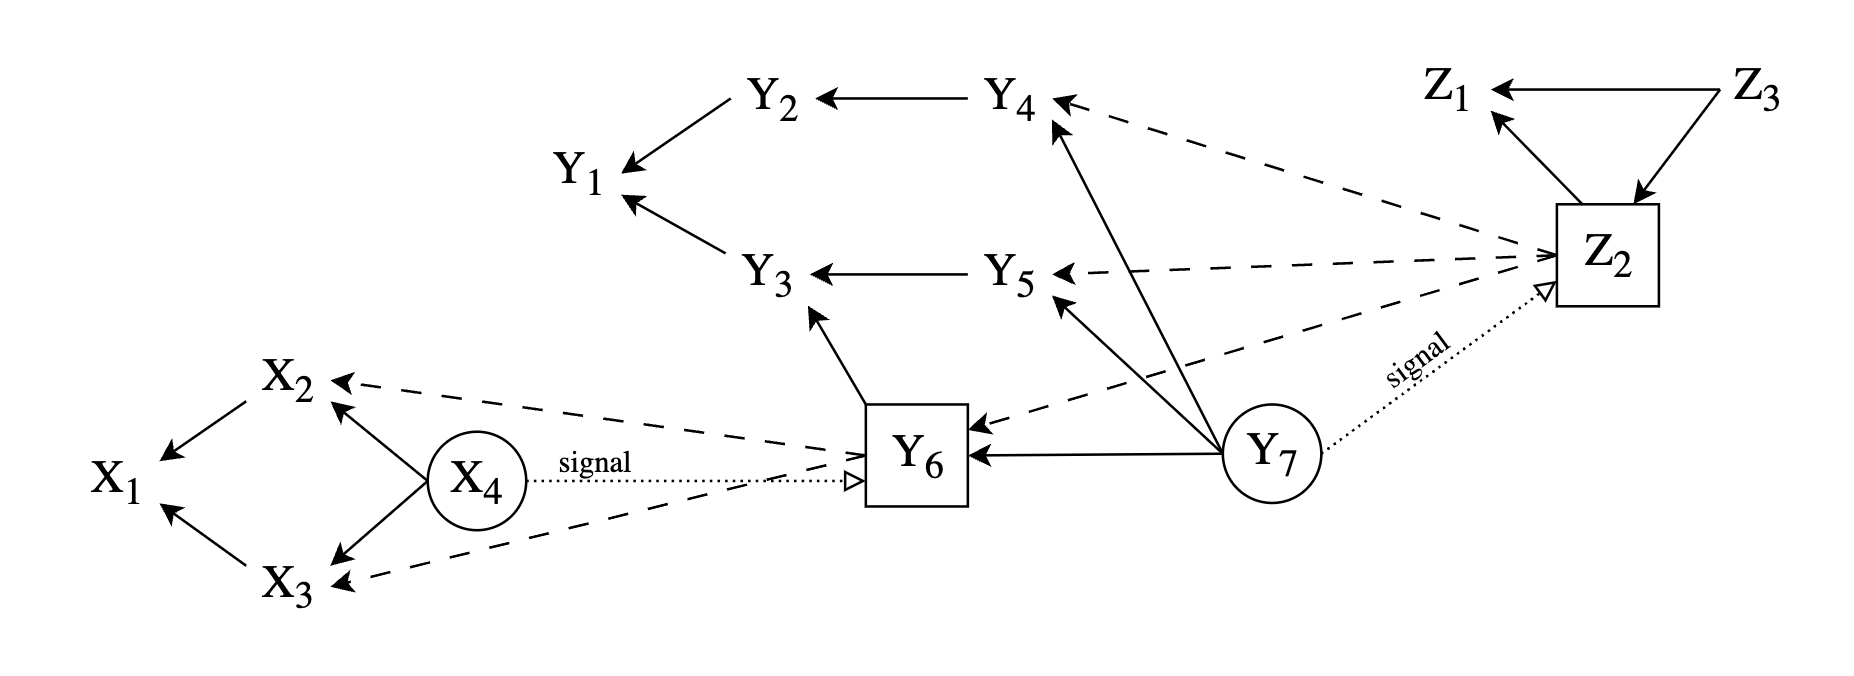
\includegraphics[width=15cm]{fig4}
    \caption{Hash graphs of CRO $X$, $Y$, $Z$ interacting by passing signals (original states are omitted). Cross-object signals are denoted as dotted arrows. Cross-object causal dependencies are denoted as dashed pointers. The vertices where signals are originated are enclosed in circles, whereas those on the receiving sides are enclosed in squares. In this example, the generation of vertex $X_4$ also produces a signal to object $Y$, materializing into vertex $Y_6$. Signaling also occurred between vertices $Y_7$ and $Z_2$. The causal dependencies of $Y_6$ is $X_2$, $X_3$, and $Y_3$. The causal dependencies of $Z_2$ is $Y_4$, $Y_5$, $Y_6$, and $Z_1$.}
    \label{fig:4}
\end{figure}

\section{Invariants}
\label{sec:headings}

Besides composability, preservation of invariants of all kinds is crucial for CROs to be richly expressive. An invariant in a distributed system is a predicate over the system state or state transitions that is always true, observed at any of its replicas. Consider two types of invariants:
\begin{enumerate}
    \item \textit{Numeric invariants}. For example, a numeric invariant required for cryptocurrency applications is that an account balance is nonnegative at all times. This invariant could break down when we allow concurrent updates to the same account — a shared wallet with \$1 left, spent concurrently by Alice and Bob.
    \item \textit{Integrity invariants}. For example, referential integrity requires that if there is a pointer from object A to B, B must be valid. This invariant is compromised when a new reference to B is added while B is invalidated concurrently.
\end{enumerate}

Common approaches to preserving such invariants include:
\begin{enumerate}
    \item \textit{Reservation}. Reservation assigns each replica the right to perform certain operations in advance \cite{Bounded-CRDT}. For example, a wallet of an initial balance \$2N may give Alice and Bob each the right to spend exactly \$N.
    \item \textit{Compensation}. Compensation repairs the violation of invariants by performing additional operations \cite{IPA}. Using the same wallet example, when a replica detects a negative balance, it may generate a compensation operation that invalidates one or some of the latest spend operations following a deterministic policy, restoring the account balance back to nonnegative. All honest replicas follow the same policy, guaranteeing convergence. In the case of referential integrity, when a replica detects the invalidated object B was concurrently referred to by another operation, it may generate a compensation operation that restores the validity of object B but sets its content to null.
\end{enumerate}

\section{Examples}
\label{sec:headings}

In this section, we provide two examples that illustrate the expressivity of CRO.

\subsection{Example 1}

The first example is a social graph that demonstrates the composability of CROs. Algorithm 1 shows the pseudocode of a blueprint named GMapGSet, which is a grow-only map (GMap) where values are grow-only sets (GSets). When adding a key-value pair to it, the pair is inserted into the map if the key is absent, otherwise the value is added to the GSet corresponding to the key in the map.

\begin{algorithm}
\caption{GMapGSet}
\begin{algorithmic}
\State \textbf{state:}
\State \hspace{\algorithmicindent} $Map$ : GMap$<$any $\Rightarrow$ GSet$>$
\State
\State \textbf{interface:}
\State \hspace{\algorithmicindent} \textbf{signal} $Add\,(k$ : any$,v$ : any$)$
\State \hspace{\algorithmicindent} \textbf{function} $Get\,(k$ : any$) \rightarrow\,v$ : Set<any>
\State
\State \textbf{on signal} $Add$
\State\hspace{\algorithmicindent}$k \notin map \Rightarrow map.insert (k,v)$
\State\hspace{\algorithmicindent}$else\Rightarrow map[k].add(v)$
\State
\State \textbf{function} $Get$
\State\hspace{\algorithmicindent}\textbf{return} $map[k]$
\end{algorithmic}
\end{algorithm}

We can build a basic social graph on top of this CRO. Algorithm 2 shows the pseudocode of a blueprint named SocialGraph, which uses a GSet to store user public keys, a two-phase set (2PSet) to store posts, and instantiates the GMapGSet blueprint to store the timestamps when users are added. Note that the timestamps in the signals $AddUser$ and $AddPost$ are reported by nodes voluntarily, which can be faulty. In the next example, we drop these timestamps and leverage hash graphs for causal ordering.

\begin{algorithm}
\caption{SocialGraph}
\begin{algorithmic}
\State \textbf{state:}
\State \hspace{\algorithmicindent} $Users$ : GSet$<$User$>$ \Comment{Grow-only set; built-in}
\State \hspace{\algorithmicindent} $Posts$ : 2PSet$<$Post$>$ \Comment{Two-phase set; built-in}
\State \hspace{\algorithmicindent} $UserTimestamps$ : GMapGSet \Comment{The blueprint from Algorithm 1}
\State
\State \textbf{interface:}
\State \hspace{\algorithmicindent} \textbf{signal} $AddUser\,(userPublicKey$ : User$,\,timestamp$ : Timestamp $)$
\State \hspace{\algorithmicindent} \textbf{signal} $AddPost\,(post$ : Post$)$
\State \hspace{\algorithmicindent} \textbf{signal} $RemovePost\,(post$ : Post$)$
\State \hspace{\algorithmicindent} \textbf{function} $GetUsers\,() \rightarrow\, $Set$<$User$>$
\State \hspace{\algorithmicindent} \textbf{function} $GetPosts\,() \rightarrow\, $Set$<$Post$>$
\State
\State \textbf{on signal} $AddUser$
\State \hspace{\algorithmicindent} $Users.Add(userPublicKey)$
\State \hspace{\algorithmicindent} $UserTimestamps.Add(userPublicKey,\,timestamp)$
\State
\State \textbf{on signal} $AddPost$
\State \hspace{\algorithmicindent} $Posts.Add(post)$
\State
\State \textbf{on signal} $RemovePost$
\State \hspace{\algorithmicindent} $Posts.Remove(post)$
% \EndFunction
\State
\State \textbf{function} $GetUsers$
\State \hspace{\algorithmicindent}\textbf{return} $Users.Set$
\State
\State \textbf{function} $GetPosts$
\State \hspace{\algorithmicindent}\textbf{return} $\{$
\State \hspace{\algorithmicindent}\hspace{\algorithmicindent} $p, \forall p \in Posts.AddSet \,\land\, p \not\in Posts.RemoveSet \,\land\, p.user \in Users.Set$
\State \hspace{\algorithmicindent}\hspace{\algorithmicindent} $ \land\, p.timestamp > UserTimestamps.Get(p.user).max()$
\State \hspace{\algorithmicindent}$\}$
\State \Comment{the post needs to (1) survive in the add set,}
\State \Comment{(2) be added by a recognized user after the user was added}
\State
\State \textbf{function} $Merge\,(replica)$
\State \hspace{\algorithmicindent} $Users \leftarrow Users \cup replica.Users$\Comment{union operator is defined for 2PSet} 
\State \hspace{\algorithmicindent} $Posts \leftarrow Posts \cup replica.Posts$
\end{algorithmic}
\end{algorithm}

\begin{algorithm}
\caption{Multiplayer2DPhysics}
\begin{algorithmic}
\State \textbf{state:}
\State \hspace{\algorithmicindent} $history$ : HashGraph
\State
\State \textbf{interface:}
\State \hspace{\algorithmicindent} \textbf{signal} $Drive\,(id$ : Player$,\,dv$ : Vec2$)$\Comment{Vec2 is a 2d vector of numbers}
\State \hspace{\algorithmicindent} \textbf{signal} $Tick\,(id$ : Player$)$
\State \hspace{\algorithmicindent} \textbf{function} $GetPlayerPhysicsStates\,() \rightarrow\, $Map$<$Player$\Rightarrow$Vec2$>$, Map$<$Player$\Rightarrow$Vec2$>$
\State\Comment{One map for positions, the other map for velocities}
\State
\State \textbf{on signal} $Drive$
\State \hspace{\algorithmicindent} $history.Add(Drive(id,dv))$
\State
\State \textbf{on signal} $Tick$
\State \hspace{\algorithmicindent} $history.Add(Tick(id))$
\State \hspace{\algorithmicindent} $\_EnforceConstraints()$
\State
\State \textbf{function} $\_EnforceConstraints$
\State \hspace{\algorithmicindent} $P,\,V \,\leftarrow\, GetPlayerPhysicsStates()$
\State \hspace{\algorithmicindent} if $\neg \_hasOverlap(P)$ \textbf{return} \Comment{$\_hasOverlap$ checks for overlapping circles}
\State \hspace{\algorithmicindent} $V_{comp} \leftarrow \_ComputeCompensation(P,V)$
\State \hspace{\algorithmicindent} $\forall (id,v) \in V_{comp} \,\{$
\State \hspace{\algorithmicindent} \hspace{\algorithmicindent} $history.Add(Compensate(id, v))$
\State \hspace{\algorithmicindent} $\}$
\State
\State \textbf{function} $GetPlayerPhysicsStates$
\State \hspace{\algorithmicindent} $operations \leftarrow history.serialize(Compensate > Drive, Tick)$
\State \Comment{serialize by topological sort; $Compensate$ wins in case of concurrency}
\State \hspace{\algorithmicindent} $P \leftarrow InitialPlayerPositions$
\State \hspace{\algorithmicindent} $V \leftarrow InitialPlayerVelocities$
\State \hspace{\algorithmicindent} $\forall op \in operations \,\{$
\State \hspace{\algorithmicindent}\hspace{\algorithmicindent} $type(op) = Drive \Rightarrow V[op.id] \leftarrow V[op.id] + op.dv$
\State \hspace{\algorithmicindent}\hspace{\algorithmicindent} $type(op) = Compensate \Rightarrow V[op.id] \leftarrow op.v$
\State \hspace{\algorithmicindent}\hspace{\algorithmicindent} $type(op) = Tick \Rightarrow P[op.id] \leftarrow P[op.id] + V[op.id] * DT$
\State \Comment{$DT$ is the constant time difference}
\State \hspace{\algorithmicindent} $\}$
\State \hspace{\algorithmicindent} \textbf{return} $P,\,V$
\State
\State \textbf{function} $Merge\,(replica)$
\State \hspace{\algorithmicindent} $history \leftarrow history \cup replica.history$ \Comment{union operator is defined for HashGraph}
\State \hspace{\algorithmicindent} $\_EnforceConstraints()$
\end{algorithmic}
\end{algorithm}

\subsection{Example 2}

The second example is a multiplayer physics simulation that demonstrates the compensation technique and the use of hash graph. For simplicity, we construct a 2D space where players move around in the form of circle objects that collide elastically with one another. These circle objects have random radii and masses, whose values are determined when players join the space. The physics state of each object contains a position vector and a velocity vector. The goal is to design a blueprint that describes this construction.

We start by specifying two types of operations, \textit{Drive} and \textit{Tick}. Drive applies a change to the velocity vector of an object. Tick advances the time of an object, which causes its position to change by velocity times a constant time difference. Objects are driven and ticked only by the players that control them.

Traversing a hash graph containing such operations, we can obtain for each player a sequence of operations they generated. To compute the position of a particular player, we traverse their sequence of operations, updating the velocity when we encounter a Drive operation, and updating the position by adding a displacement to it when we encounter a Tick operation. The displacement is equal to the product of the velocity and the constant time difference. 

However, the above construction does not consider the elastic collision constraints. Geometrically, a collision between two objects occurs when their shapes overlap. Equation 1 expresses the no-overlap constraint for two circles $i$ and $j$, where $(x,y)$ refers to the center of a circle, and $r$ refers to its radius. Clearly, this is a numeric invariant that can be violated by concurrent positional changes of the circles. Equation 2 expresses the elastic collision constraint between two circles $i$ and $j$, where their relative velocites along the normal direction before and after the collision are $v^-_{rel}$ and $v^+_{rel}$ respectively, and $e$ is a scalar representing the restitution coefficient.

\begin{equation}
(x_i-x_j)^2 + (y_i-y_j)^2 \,\geq\, (r_i + r_j)^2
\end{equation}

\begin{equation}
v^+_{rel} = -e \cdot v^-_{rel}
\end{equation}

We adopt the compensation technique to enforce both the no-overlap constraint and the perfect elastic collision constraint. A new type of operation is introduced, \textit{Compensate}, which directly sets the velocities of the colliding circles to new values in order to repair constraint violation. To ensure convergence, we also introduce the semantics that \textit{Compensate} wins in case it is concurrent to \textit{Drive} or \textit{Tick} that attempts to mutate the velocities of the same circles.  Many approaches exist for computing these compensating velocity values, such as the sequential impulse approach \cite{Jakobsen, Guendelman} and the Linear Complementarity Problem (LCP) approach \cite{LCP, Box2D}. The details of these approaches are outside of the scope of this paper. This construction has a number of issues, including tunneling (\textit{i.e., } when two objects pass through each other without overlapping at any tick) and players ticking at different rates. How to modify the construction to handle these issues is beyond the scope of this paper.

Algorithm 3 shows the pseudocode of a blueprint named Multiplayer2DPhysics, illustrating the construction above. By having $\_ComputeCompensation$ a fully deterministic procedure, we can ensure that all honest replicas will generate the exact same compensations, guaranteeing convergence.

\section{Interaction methods}
\label{sec:headings}

Topology Protocol defines a set of methods, or simply \textit{verbs}, for nodes to interact with a given CRO. At the core of the protocol is the PubSub model for nodes in P2P networks to subscribe to CROs and publish updates on them asynchronously. CROs are identified as PubSub groups or topics. Nodes only subscribe to CROs they are interested in. This keeps CROs loosely coupled and helps reduce memory and bandwidth requirement for operating nodes. In contrast, every network participant of a blockchain is by default "subscribed" to all smart contracts. Figure 5 illustrates this interaction pattern.

\begin{figure}[htp]
    \centering
    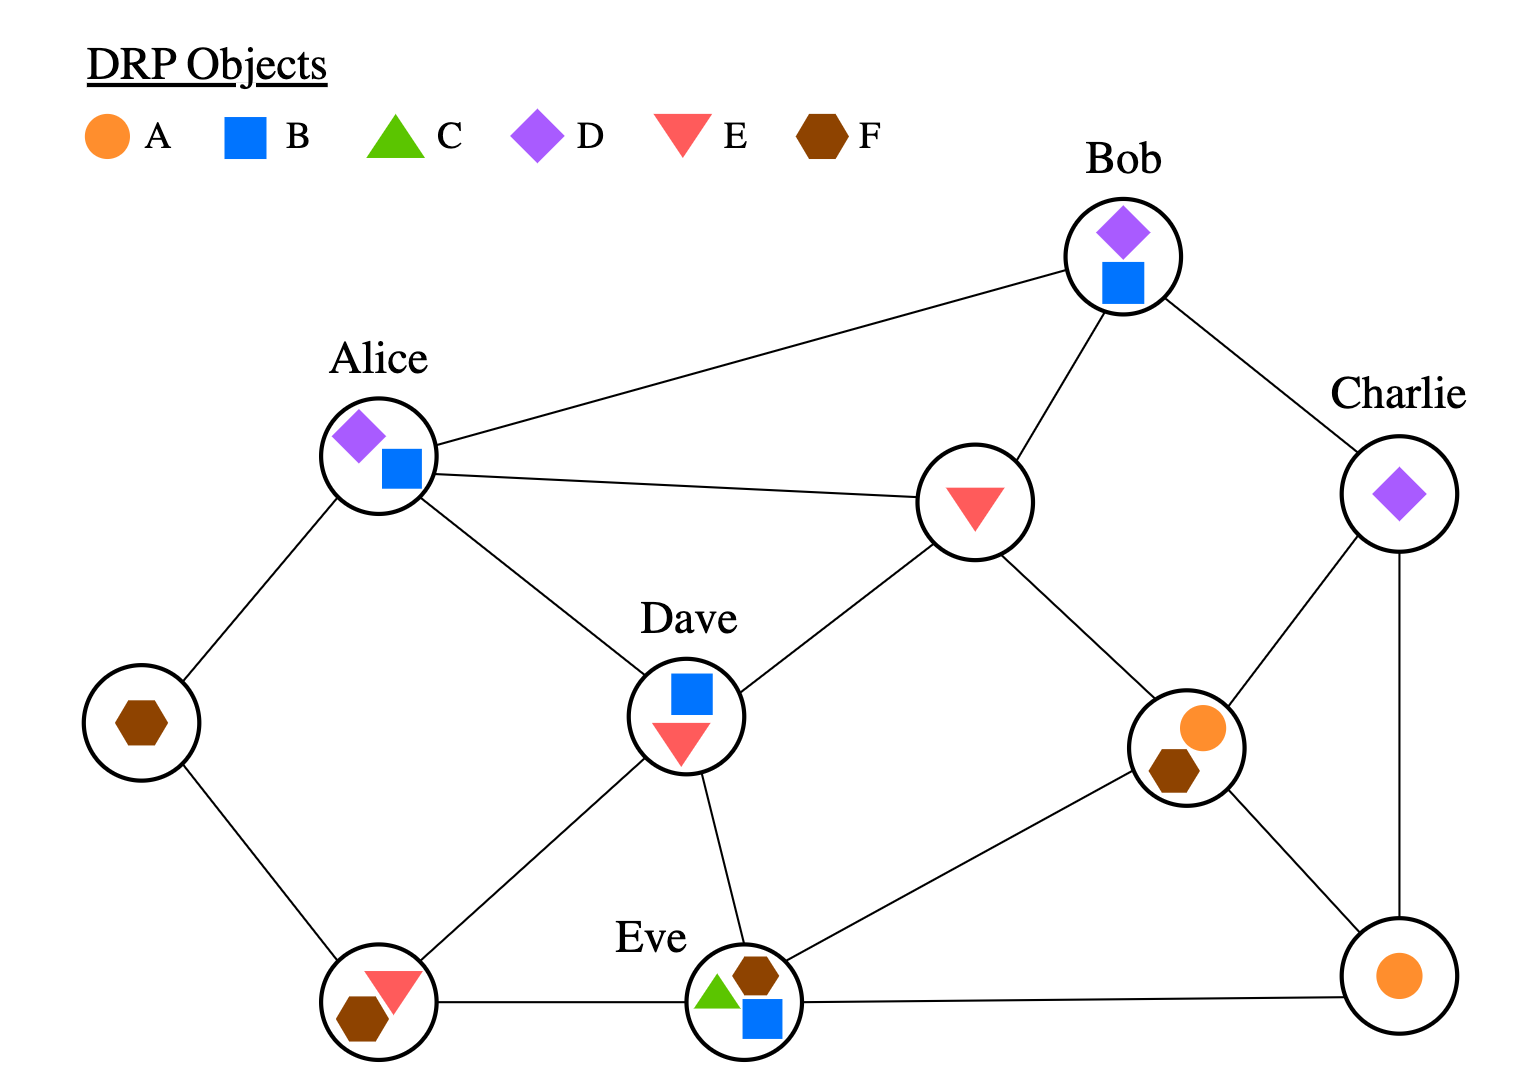
\includegraphics[width=13cm]{fig5}
    \caption{Alice, Bob, and Charlie are subscribed to CRO $D$. Alice, Bob, Dave, and Eve are subscribed to CRO $B$. All nodes are connected peer-to-peer.}
    \label{fig:5}
\end{figure}

The set of core interaction methods and their semantics is as follows:
\begin{enumerate}
    \item \textbf{CREATE}: to create a new CRO. Under the hood, a PubSub group (topic) is created for the new CRO.
    \item \textbf{UPDATE}: to perform an update operation on a given CRO. The update is published to the corresponding PubSub group.
    \item \textbf{SUBSCRIBE}: to subscribe to all updates performed on a given CRO. The node adds the corresponding PubSub group to its groups of interest.
    \item \textbf{UNSUBSCRIBE}: to unsubscribe and stop receiving updates on a given CRO. The node removes the corresponding PubSub group from its groups of interest.
    \item \textbf{SYNC}: to reconcile the differences in operation histories (hash graphs) of a given CRO between the local one and a remote one. The SYNC method has two main purposes: for a new node to bootstrap into an existing CRO, and as an out-of-band synchronization method besides P2P gossiping.
\end{enumerate}

SYNC can take a long time to complete when a node is bootstrapping into a CRO with a large history. This can be viewed as a problem of set reconciliation. One common approach is to exchange bloom filters to reduce the message complexity of the sync process. A more promising approach has constant overhead even when reconciling sets with very large differences \cite{PRIBLT}.

\section{Operation life cycle}
\label{sec:headings}

The life cycle of a CRO operation differs significantly from a blockchain transaction. When a node performs a write (update) by generating an operation on a CRO, the operation is added to the node's local copy of the CRO's hash graph immediately. A node reads a CRO state by serializing the node's local copy of the CRO's hash graph. If a node performs a write and a subsequent read immediately, the read is guaranteed to observe the write. In other words, CRO provides highly available operations and guarantees low latency \cite{HAT}. In contrast, blockchains are not highly available. A blockchain transaction becomes available only after it is included in a block that is proposed, verified and acknowledged by a threshold amount of network participants.

\section{Snapshot}
\label{sec:headings}

A CRO snapshot is a single hash graph that represents an agreement among the CRO's replicas. It serves multiple purposes:
\begin{enumerate}
    \item It acts as a "state save" that may be worth persisted (\textit{e.g.}, on IPFS \cite{IPFS}).
    \item It can be used to generate irreversible transactions on blockchains.
\end{enumerate}

The computation of snapshots faces several problems. We must avoid involving "all nodes" in the algorithm: unanimity can be very problematic due to network conditions, dynamic membership, and Byzantine behavior. The algorithm needs to run concurrently to the underlying CRO activities without hindering or suspending them. The algorithm must complete with reasonable bandwidth consumption, thus the nodes involved must not send entire replicas over the wire.

Our current solution builds on threshold logical clock (TLC) \cite{TLC} as a decentralized pacemaker, on top of which Byzantine consensus can be reached. Each CRO has its own TLC operated by its subscriber nodes. When a node is ready to advance the TLC tick, it proposes the hashed frontier $\textbf{F}^*$ of its own hash graph by broadcasting it to other subscribers. Instead of unanimity, the tick advances by threshold amounts of subscriber nodes signing and acknowledging messages. Three consecutive ticks can be used to form a consensus round, yielding a snapshot. The process runs continuously, allowing snapshots to be taken periodically.

CRO snapshots remain an active area of research. The algorithms and their configurability supported by the protocol remain to be determined through the protocol development process.

\section{Compaction}
\label{sec:headings}

Grow-only hash graphs are problematic. Unbounded memory is needed, and large graphs take longer to bootstrap. Compaction serializes the state of a CRDT by applying the operations carried by a portion of the hash graph before pruning that portion away. Compaction discards causal information and thus is perfectly safe only when performed over vertices that will never be the causal dependencies of any future operations.

However, perfectly safe compaction can be impractical. To be certain that a vertex $V$ is perfectly safe to drop, a node needs to receive a vertex from every other node that causally depends on $V$ \cite{PO-CRDT}. This involves the notion of "all nodes", our usual suspect. Our current solution is to use the TLC consensus rounds to drive compaction. Each round yields a hash graph, whose frontier $\textbf{F}$ comprises vertices that are considered causally stable. All preceding vertices can be compacted. The CRO's state is forwarded by applying the operations of those compacted vertices in a linear order obtained from topological sort. Figure 6 illustrates this process.

\begin{figure}[htp]
    \centering
    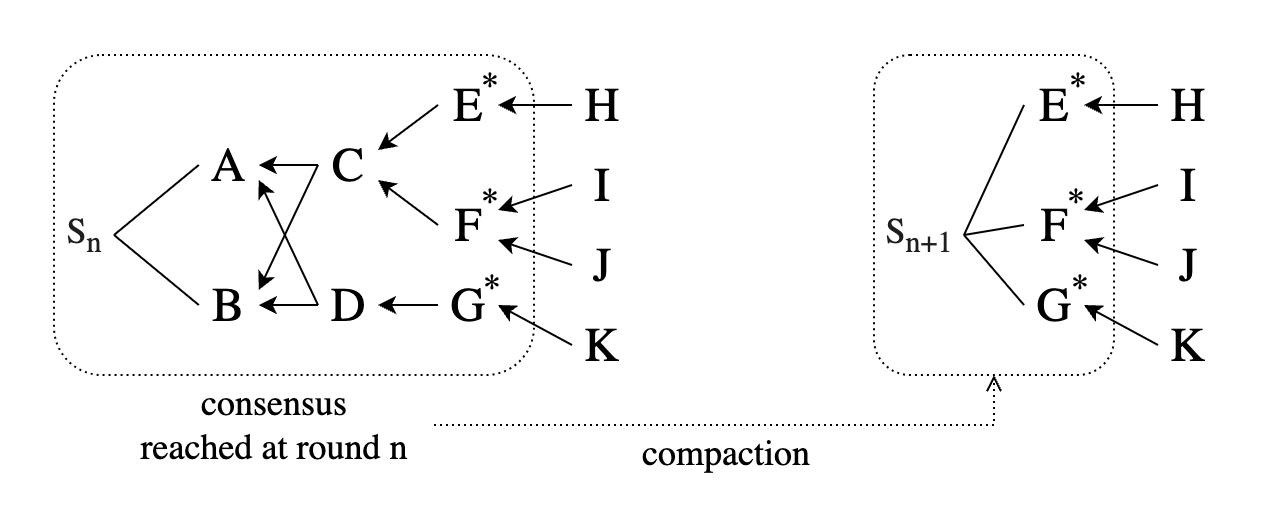
\includegraphics[width=13cm]{fig6}
    \caption{Compaction is performed on the subgraph containing vertices $A,B,C,D$ that precedes the frontier $\textbf{F}$ of the hash graph decided by consensus. The vertices in the frontier $\textbf{F}$ of the hash graph before compaction are marked with asterisks $*$, which form the origin $\textbf{O}$ of the hash graph after compaction. $S_{n+1}$ is computed by applying the operations in the subgraph on $S_n$ in a linear order obtained from topological sort.}
    \label{fig:6}
\end{figure}

Unsafe compaction is named as such because it may drop causal information in the hash graph that is needed to recognize the causality of operations that have yet to arrive from the network. Thus, operations with unrecognizable causality could come from both honest and Byzantine nodes. Existing approaches from Tusk \cite{Tusk} and Bullshark \cite{Bullshark} choose to re-inject transactions in a later consensus round. These approaches aim to preserve some notion of fairness, ensuring that transactions generated by correct nodes are eventually delivered to all other correct nodes. However, re-injected transactions lose their original causal dependencies, requiring rewriting on top of the hash graph frontier from the previous consensus round. A consistent, deterministic policy for rewriting dependencies is needed. Compaction remains an active area of research.

Revisiting the snapshot problem, we can see why producing grow-only snapshots is undesirable. Using compaction, we can shrink the size of a snapshot. This is particularly valuable when snapshots are to be stored on blockchains, where storage is expensive.

By leveraging recursive zero-knowledge proofs \cite{Recursive-SNARK}, it is possible to produce compacted snapshots that are verifiable, which are useful in scenarios where trust needs to be minimized. A compacted snapshot is verifiable when anyone can verify that (1) consensus was reached correctly (2) compaction was performed correctly. For the consensus part, we can require the proposals in each round to contain the hash of the agreed upon proposal and the aggregated signatures from the previous round. This effectively forms a chain. Verifying the aggregated signatures at the tip of the chain verifies the entire chain. For the compaction part, we can require the blueprint to be executable by a provable VM such as Cairo \cite{Cairo}, RISC0 \cite{RISC0}, or Valida \cite{Valida}. The state forwarding step of compaction can be proven recursively, yielding a recursive proof that sits alongside the snapshot.


\section{Access control}
\label{sec:headings}

Access control is important for multiplayer applications. Social and communal spaces are much more useful when fine-grained permissions can be assigned to participants. Common access control models include level-based (lattice-based) \cite{LBAC} and role-based ones \cite{RBAC}. It gets tricky when a CRO's access control logic is specified within itself or another CRO, due to eventual consistency. What happens when an operation that revokes the access role of a participant is concurrent to an operation generated by the same participant that depends on having the very role assigned?

The core issue here is conflict resolution strategies that involve permission changes. A promising solution is proposed in \cite{Matrix}, where both permission roles or levels and the causal order among operations are taken into account to topologically sort a hash graph. The solution works under the assumption that participants with higher permission roles or levels are not attackers. Another promising direction is to leverage the TLC to establish a linear order between permission-changing operations and permission-dependent operations. A CRO may require that permission-changing operations remain ineffective until the next TLC tick.

\section{Security}
\label{sec:headings}

Security is a critical aspect of CROs. We consider three threat models for CROs and explore potential solutions.

\subsection {Hash graph pollution}
Hash graphs can be polluted by vertices with garbage payload such as invalid operations. When receiving a new vertex, a node can validate its operation before adding it to the local hash graph. The nodes that published bad operations can be banned. If an operation can be validated atomically, we can be certain that all honest nodes will reach the same conclusion. It is trickier when the validity of the operation depends on the operations that happened before it. In this case, we can define operation validity as a function of the operation itself and all operations that can be transitively reached through the causal dependencies in the hash graph \cite{BFT-CRDT}.

\subsection {Equivocation}
Equivocation occurs when a node, assumed to be a single-threaded process, generates concurrent operations. An honest node can detect that another node has generated concurrent operations. The honest node may choose to remove the corresponding bad vertices from its hash graph, ban the Byzantine node, and expect all other honest nodes to do the same. However, downstream vertices that causally depend on these bad vertices may have been generated. It is not obvious how to graft these downstream vertices back to the hash graph. Equivocation tolerance remains an active area of research.

\subsection {Backdated dependencies}
We consider this as the trickiest threat model: when nodes report dependencies that are older than the vertices in the frontier. The question is how backdated dependencies can be reliably detected by all honest nodes. A vertex carrying correct dependencies but arriving late due to network delays is indistinguishable from a vertex with backdated dependencies. One promising direction is to leverage the TLC as it introduces a notion of linear time. Denote the frontier of the hash graph from $n$ consensus rounds ago as $\textbf{F}_{-n}$. A CRO can stipulate that a vertex should not report causal dependencies that causally precede any of the vertices in $\textbf{F}_{-n}$ with $n$ carefully chosen, otherwise the vertex will be handled according to some policy that is applied consistently across all honest nodes. As such, the TLC serves as a security clock for the CRO, whose $\textbf{F}_{-n}$ serves as the backstop for backdated dependencies.

\section{Decentralized random access memory}
\label{sec:headings}

A compelling perspective on Topology Protocol is its ability to power a decentralized network that functions as a "decentralized Random Access Memory" (dRAM). The following properties of the protocol support this perspective:

\begin{enumerate}
    \item \textbf{Random access}. Users can synchronize on any CROs of interest without having to synchronize every single CRO in the system, contrary to smart contracts on blockchains. This access pattern reduces the resource requirement of running a protocol node, making it more accessible for users to participate in the network.
    \item \textbf{Closeness to compute}. We envision that most users of CRO-powered applications will operate nodes on their devices, holding CRO replicas locally. In other words, the protocol champions the principles of local-first software \cite{LoFi}. This approach reduces latency, enhances privacy, and improves both scalability and resilience by "load-balancing" across user devices. In contrast, most blockchain users access smart contracts via centralized RPC nodes, not unlike the access pattern of most cloud apps. This property is analogous to the role random access memory serves in a memory hierarchy.
    \item \textbf{Ephemerality}. Persistence of CROs is out of scope of the protocol. The protocol expects the nodes to be ephemeral. Their states are volatile from the system's perspective, corresponding to the volatility of RAM. The data movement between Topology nodes and persistence providers is analogous to the data movement between RAM and disk storage which is non-volatile.
\end{enumerate}
\noindent

Decentralized RAM has the potential to enable a new class of decentralized applications that can operate more dynamically and responsively than blockchain-based applications.

\section{Conclusion}

In this paper, we introduced CRO and Topology Protocol for P2P real-time multiplayer applications. CRDT is a natural choice for such use cases, and the use of hash graphs allows capturing causality among operations while tolerating Byzantine faults. CRO provides the programmability of common object systems and encapsulates coordination-free replication strategies. Topology Protocol specifies a set of interaction methods for CROs to be created, updated, subscribed to, unsubscribed from, and synchronized. Their semantics correspond to behavior on the underlying P2P networks under the publish/subscribe model. Snapshot, compaction, access control, and threat models of CROs were addressed. Nodes that implement Topology Protocol keep replicas of CROs locally, facilitate persistence without being primarily responsible for it, and disseminate CRO updates only to nodes that are interested in them. As such, a P2P network comprised of such nodes effectively works as a decentralized RAM.

\section*{Acknowledgments}

The development of this work has been greatly enriched by the insights and support of many individuals. We would like to express our gratitude to:
\begin{itemize}[leftmargin=0.5cm]
\item Eli Ben-Sasson and Uri Kolodny, for supporting us in our endeavors to run scalable physics simulations in a decentralized manner;
\item Joon Yun, for pointing us toward the magic of CRDTs in the first place;
\item Martin Kleppmann, for the discussions on the theory behind CRDTs and the mechanics and threat models of hash graphs;
\item Zaki Manian, for discussions on the solutions to P2P connectivity issues;
\item Sina Habibian, for encouraging us to explore alternative distributed data structures on P2P networks that provide different affordances from what blockchains offer;
\item Polynya, for encouraging us to explore new software paradigms that promote the creative agency of a broad audience, and to seek alternatives to the plutocracy and oligopoly that underlie the correct functioning of all major blockchains;
\item Jihoon Song and Kunho Kim, for the original discussions that motivated this paper;
\item Jay Oak, for the pivotal input in shaping the scope and capabilities of the protocol and the abundant feedback for improving this paper;
\item Akash S M, for suggesting that we explain why concurrency semantics are important;
\item Matthew Weidner, for pointing out the challenges in exercising access control under eventual consistency, and a solution designed for the Matrix Protocol;
\item Peter van Hardenberg, for pointing out the importance of invariant preservation and suggesting that we add a representative example for discussing how constraints may be enforced in CROs;
\item Pierre Semanne and Goblin Oats, for advocating against a global finality system shared by all CROs, an idea explored in the early drafts;
\item haadcode, for reinforcing our concept of a decentralized RAM;
\item Oskar Thorén and Anderson Chen, for carefully reviewing the early drafts and offering ideas for improvement;
\item Alok Vasudev and Adam Goldberg, for the patience and encouragement for us to focus on finding the truth.
\end{itemize}

%Bibliography
\bibliographystyle{unsrt}  
\bibliography{references}  

%\lipsum[4] See Section \ref{sec:headings}.

% \subsection{Headings: second level}
% \lipsum[5]
% \begin{equation}
% \xi _{ij}(t)=P(x_{t}=i,x_{t+1}=j|y,v,w;\theta)= {\frac {\alpha _{i}(t)a^{w_t}_{ij}\beta _{j}(t+1)b^{v_{t+1}}_{j}(y_{t+1})}{\sum _{i=1}^{N} \sum _{j=1}^{N} \alpha _{i}(t)a^{w_t}_{ij}\beta _{j}(t+1)b^{v_{t+1}}_{j}(y_{t+1})}}
% \end{equation}

% \subsubsection{Headings: third level}
% \lipsum[6]

% \paragraph{Paragraph}
% \lipsum[7]

% \section{Examples of citations, figures, tables, references}
% \label{sec:others}
% \lipsum[8] \cite{kour2014real,kour2014fast} and see \cite{hadash2018estimate}.

% The documentation for \verb+natbib+ may be found at
% \begin{center}
%   \url{http://mirrors.ctan.org/macros/latex/contrib/natbib/natnotes.pdf}
% \end{center}
% Of note is the command \verb+\citet+, which produces citations
% appropriate for use in inline text.  For example,
% \begin{verbatim}
%    \citet{hasselmo} investigated\dots
% \end{verbatim}
% produces
% \begin{quote}
%   Hasselmo, et al.\ (1995) investigated\dots
% \end{quote}

% \begin{center}
%   \url{https://www.ctan.org/pkg/booktabs}
% \end{center}


% \subsection{Figures}
% \lipsum[10] 
% See Figure \ref{fig:fig1}. Here is how you add footnotes. \footnote{Sample of the first footnote.}
% \lipsum[11] 

% \begin{figure}
%   \centering
%   \fbox{\rule[-.5cm]{4cm}{4cm} \rule[-.5cm]{4cm}{0cm}}
%   \caption{Sample figure caption.}
%   \label{fig:fig1}
% \end{figure}

% \subsection{Tables}
% \lipsum[12]
% See awesome Table~\ref{tab:table}.

% \begin{table}
%  \caption{Sample table title}
%   \centering
%   \begin{tabular}{lll}
%     \toprule
%     \multicolumn{2}{c}{Part}                   \\
%     \cmidrule(r){1-2}
%     Name     & Description     & Size ($\mu$m) \\
%     \midrule
%     Dendrite & Input terminal  & $\sim$100     \\
%     Axon     & Output terminal & $\sim$10      \\
%     Soma     & Cell body       & up to $10^6$  \\
%     \bottomrule
%   \end{tabular}
%   \label{tab:table}
% \end{table}

% \subsection{Lists}
% \begin{itemize}
% \item Lorem ipsum dolor sit amet
% \item consectetur adipiscing elit. 
% \item Aliquam dignissim blandit est, in dictum tortor gravida eget. In ac rutrum magna.
% \end{itemize}


\end{document}
